The parallel implementation of FLAME seeks to use an SPMD paradigm - each node of the parallel system is running essentially the same $program$. However given the nature of agent-bsaed modelling and the FLAME implementation each nodal program could perform a very different sequence of instructions and function activations as it traverses its part of the state space. 

The two fundamental design features of FLAME are that all communications between agents takes place through a specified message board - a message respository - and that these message boards are distributed over the processing nodes of the parallel system. These message boards can be considered the data load and the agents themselves the computational load. In FLAME both these are distributed over the computational nodes.

However, although there may be some imbalance in computational load, with a reasonable initial data - agents - distribution, any imbalance should be small. The crucial element in the parallel implementation of FLAME is the distribution of the message boards over the system and their syncronisation.

Care has been taken in FLAME to overlap communication and computation so that, as far as possible, agent functions are not waiting for data during their activation. This has been acheived by FLAME analysing the sending and receiving of messages defined in the model XMML file to push the start of communication (call to \texttt{MB$\_$SyncStart()}) as high as possible in the call tree (i.e.\ just after all messages of a particular type have been sent to the message board) and the wait for communication to complete (call to \texttt{MB$\_$SyncComplete()}) as low as possible (just before the messages are required).

To illustrate the effect of overlapping communication and computation a special version of FLAME that placed the calls to  \texttt{MB$\_$SyncStart} and \texttt{MB$\_$SyncComplete} as successive operations was run alongside the usual version. The timer package was used to time the \texttt{MB$\_$SyncComplete} functions in both cases and the results are given for the 5 longest elapsed times in Figure \ref{fig:overlap}. Runs were for a 16 region problem on 2 nodes for 40 iterations. 

\begin{figure}[ht]
 \centering
  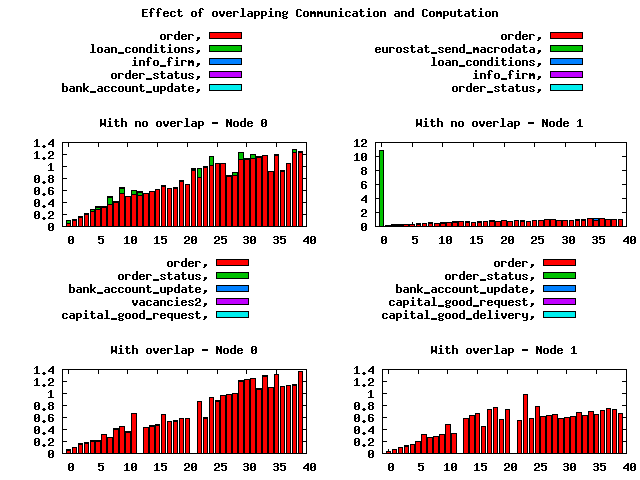
\includegraphics[width=450pt]{overlap.png}
 \caption{Elapsed times (s) for message board syncronisations with an without communication/computation overlapping}
 \label{fig:overlap}
\end{figure}

It is clear that the \texttt{eurostat$\_$send$\_$macrodata} message board is a significant beneficiary of overlapping. Looking at the state graph for the model shows that the messages are sent by the Eurostat agent very early in an iteration and read by the Government agents very late in the iteration.

The \texttt{order} message board benefits less since order messages are required very soon after they are sent (again from the state graph).

It is interesting/suprising/shocking to note that in the EURACE model even with no overlapping, all the messageboard synchronisations are only taking 5\% of the total run time.




 
